
\section{Hardware}

\begin{figure}[h]
\begin{subfigure}{.5\textwidth}
\centering
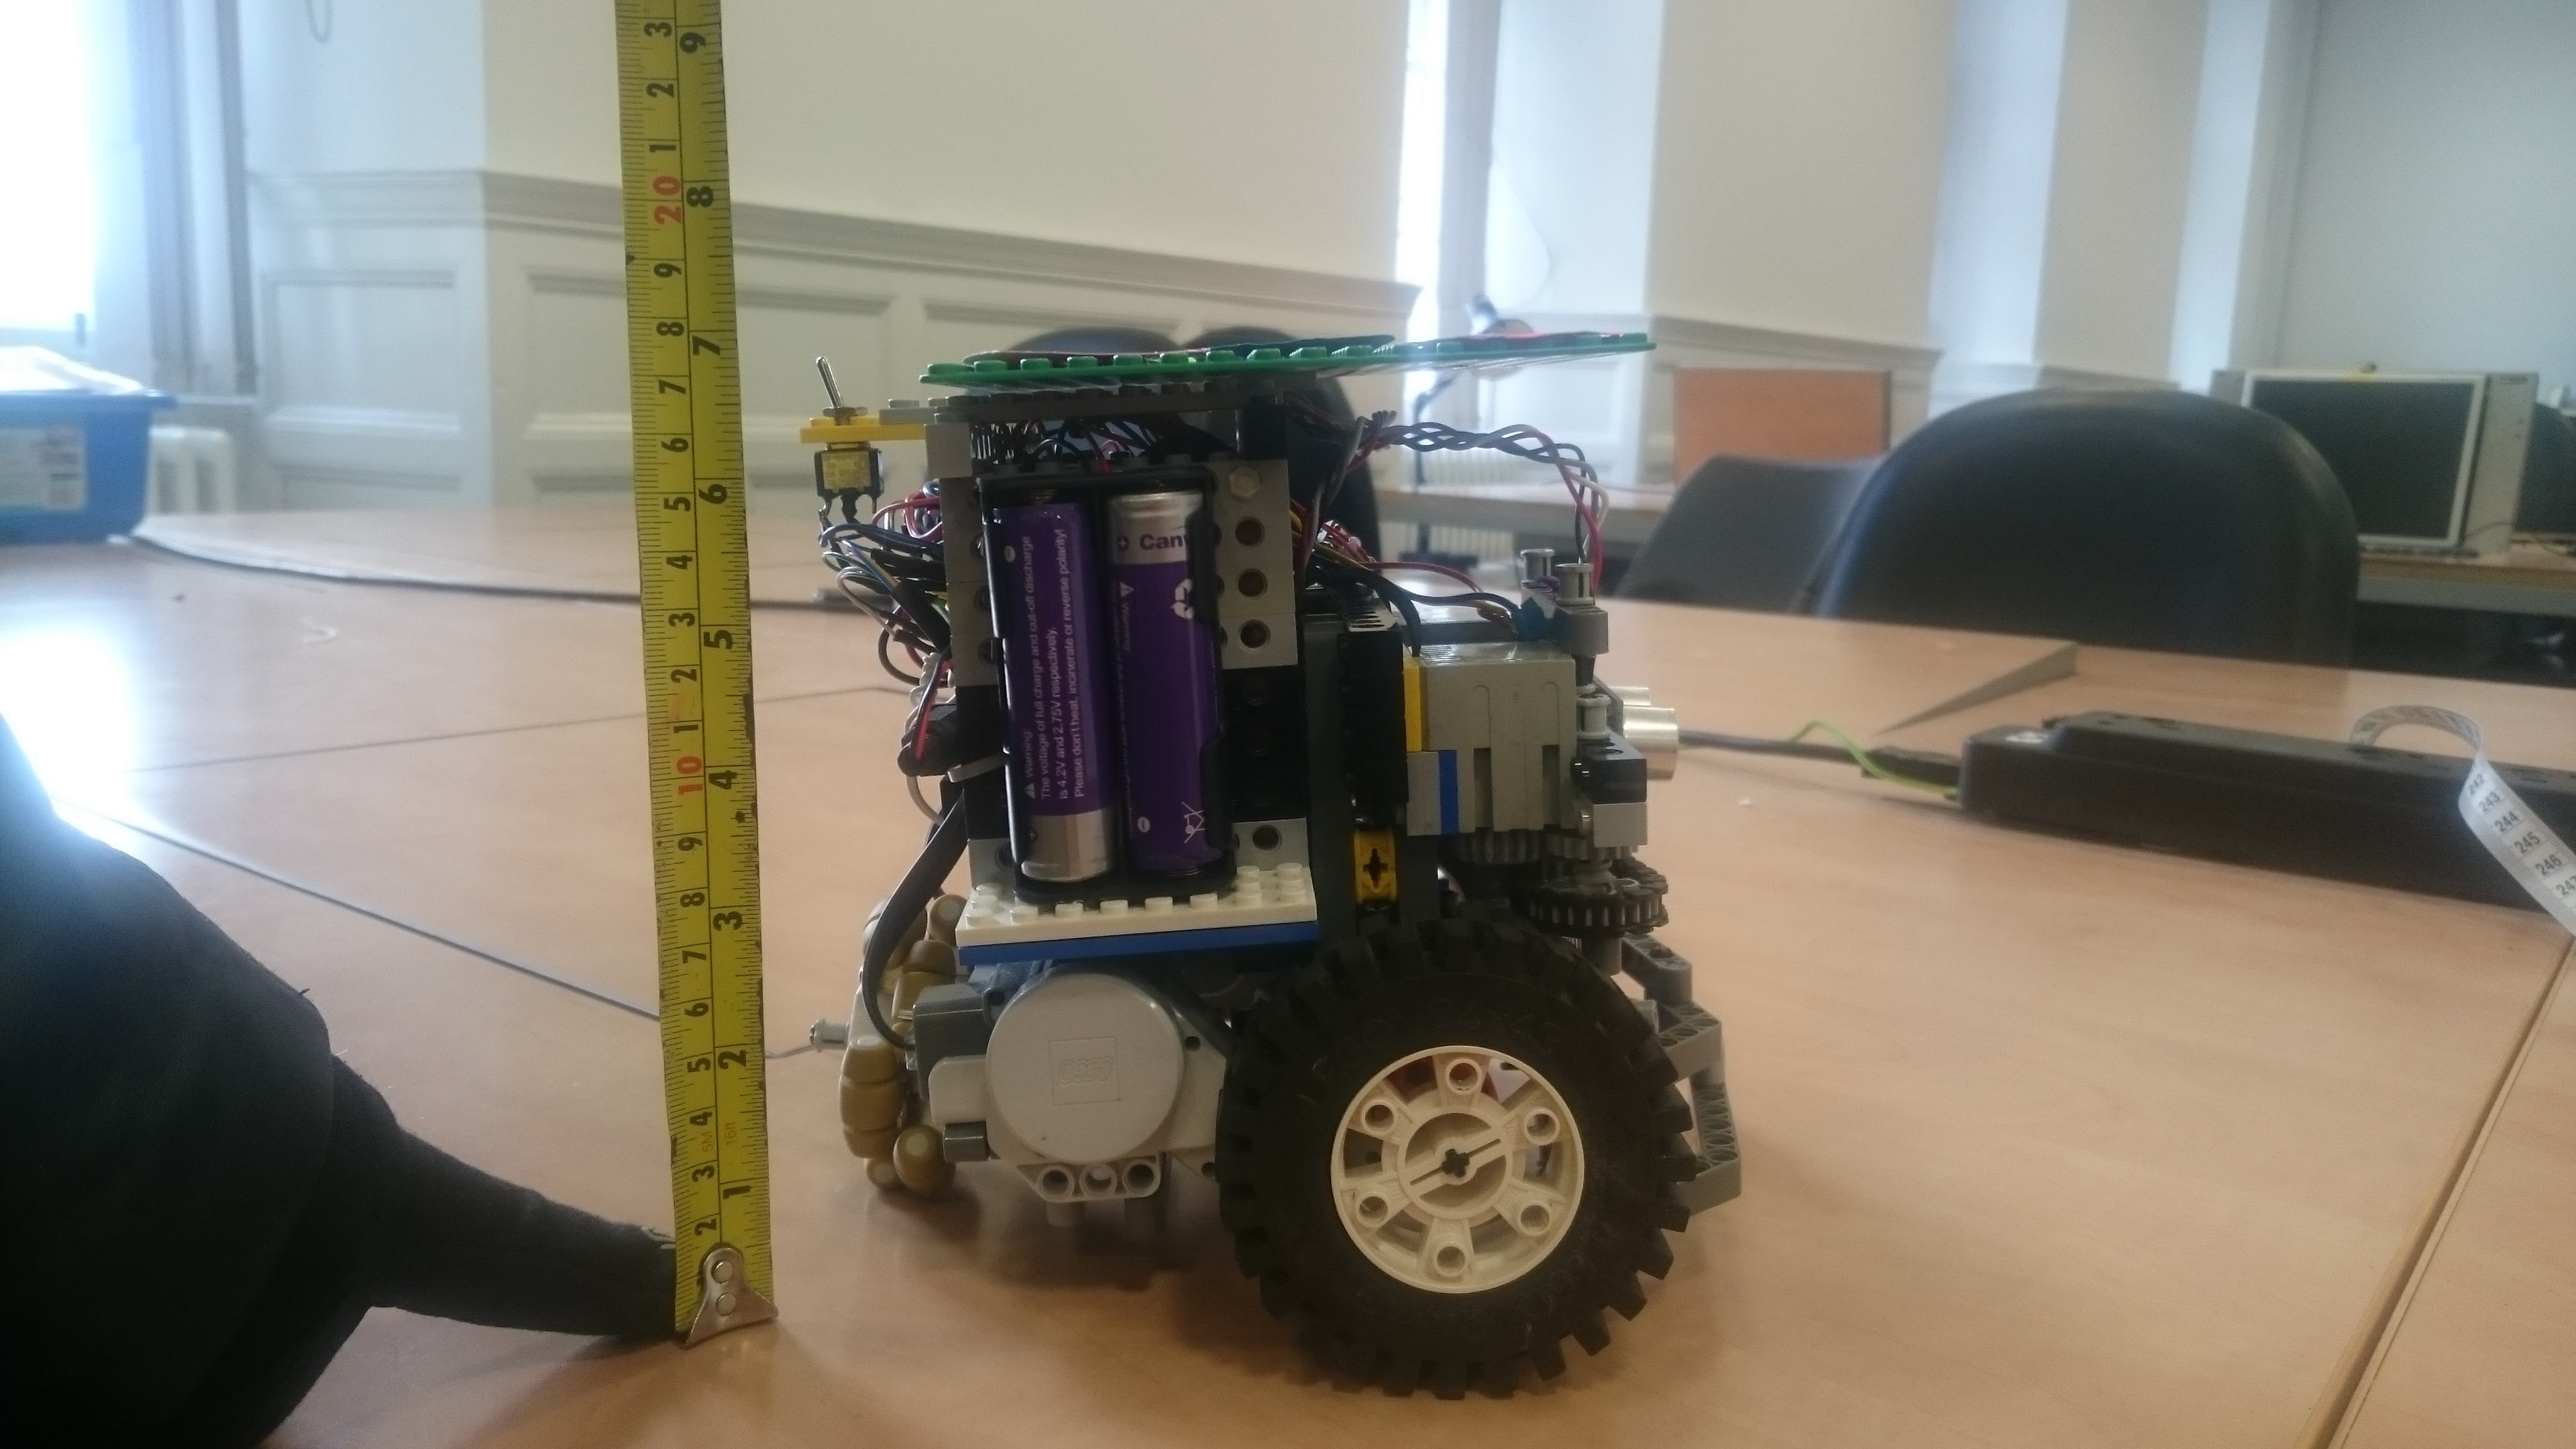
\includegraphics[width=.95\textwidth]{DSC_0148.jpg}
\caption{Side View of Robot}
\label{fig:robot_side}
\end{subfigure}%
\begin{subfigure}{.5\textwidth}
\centering
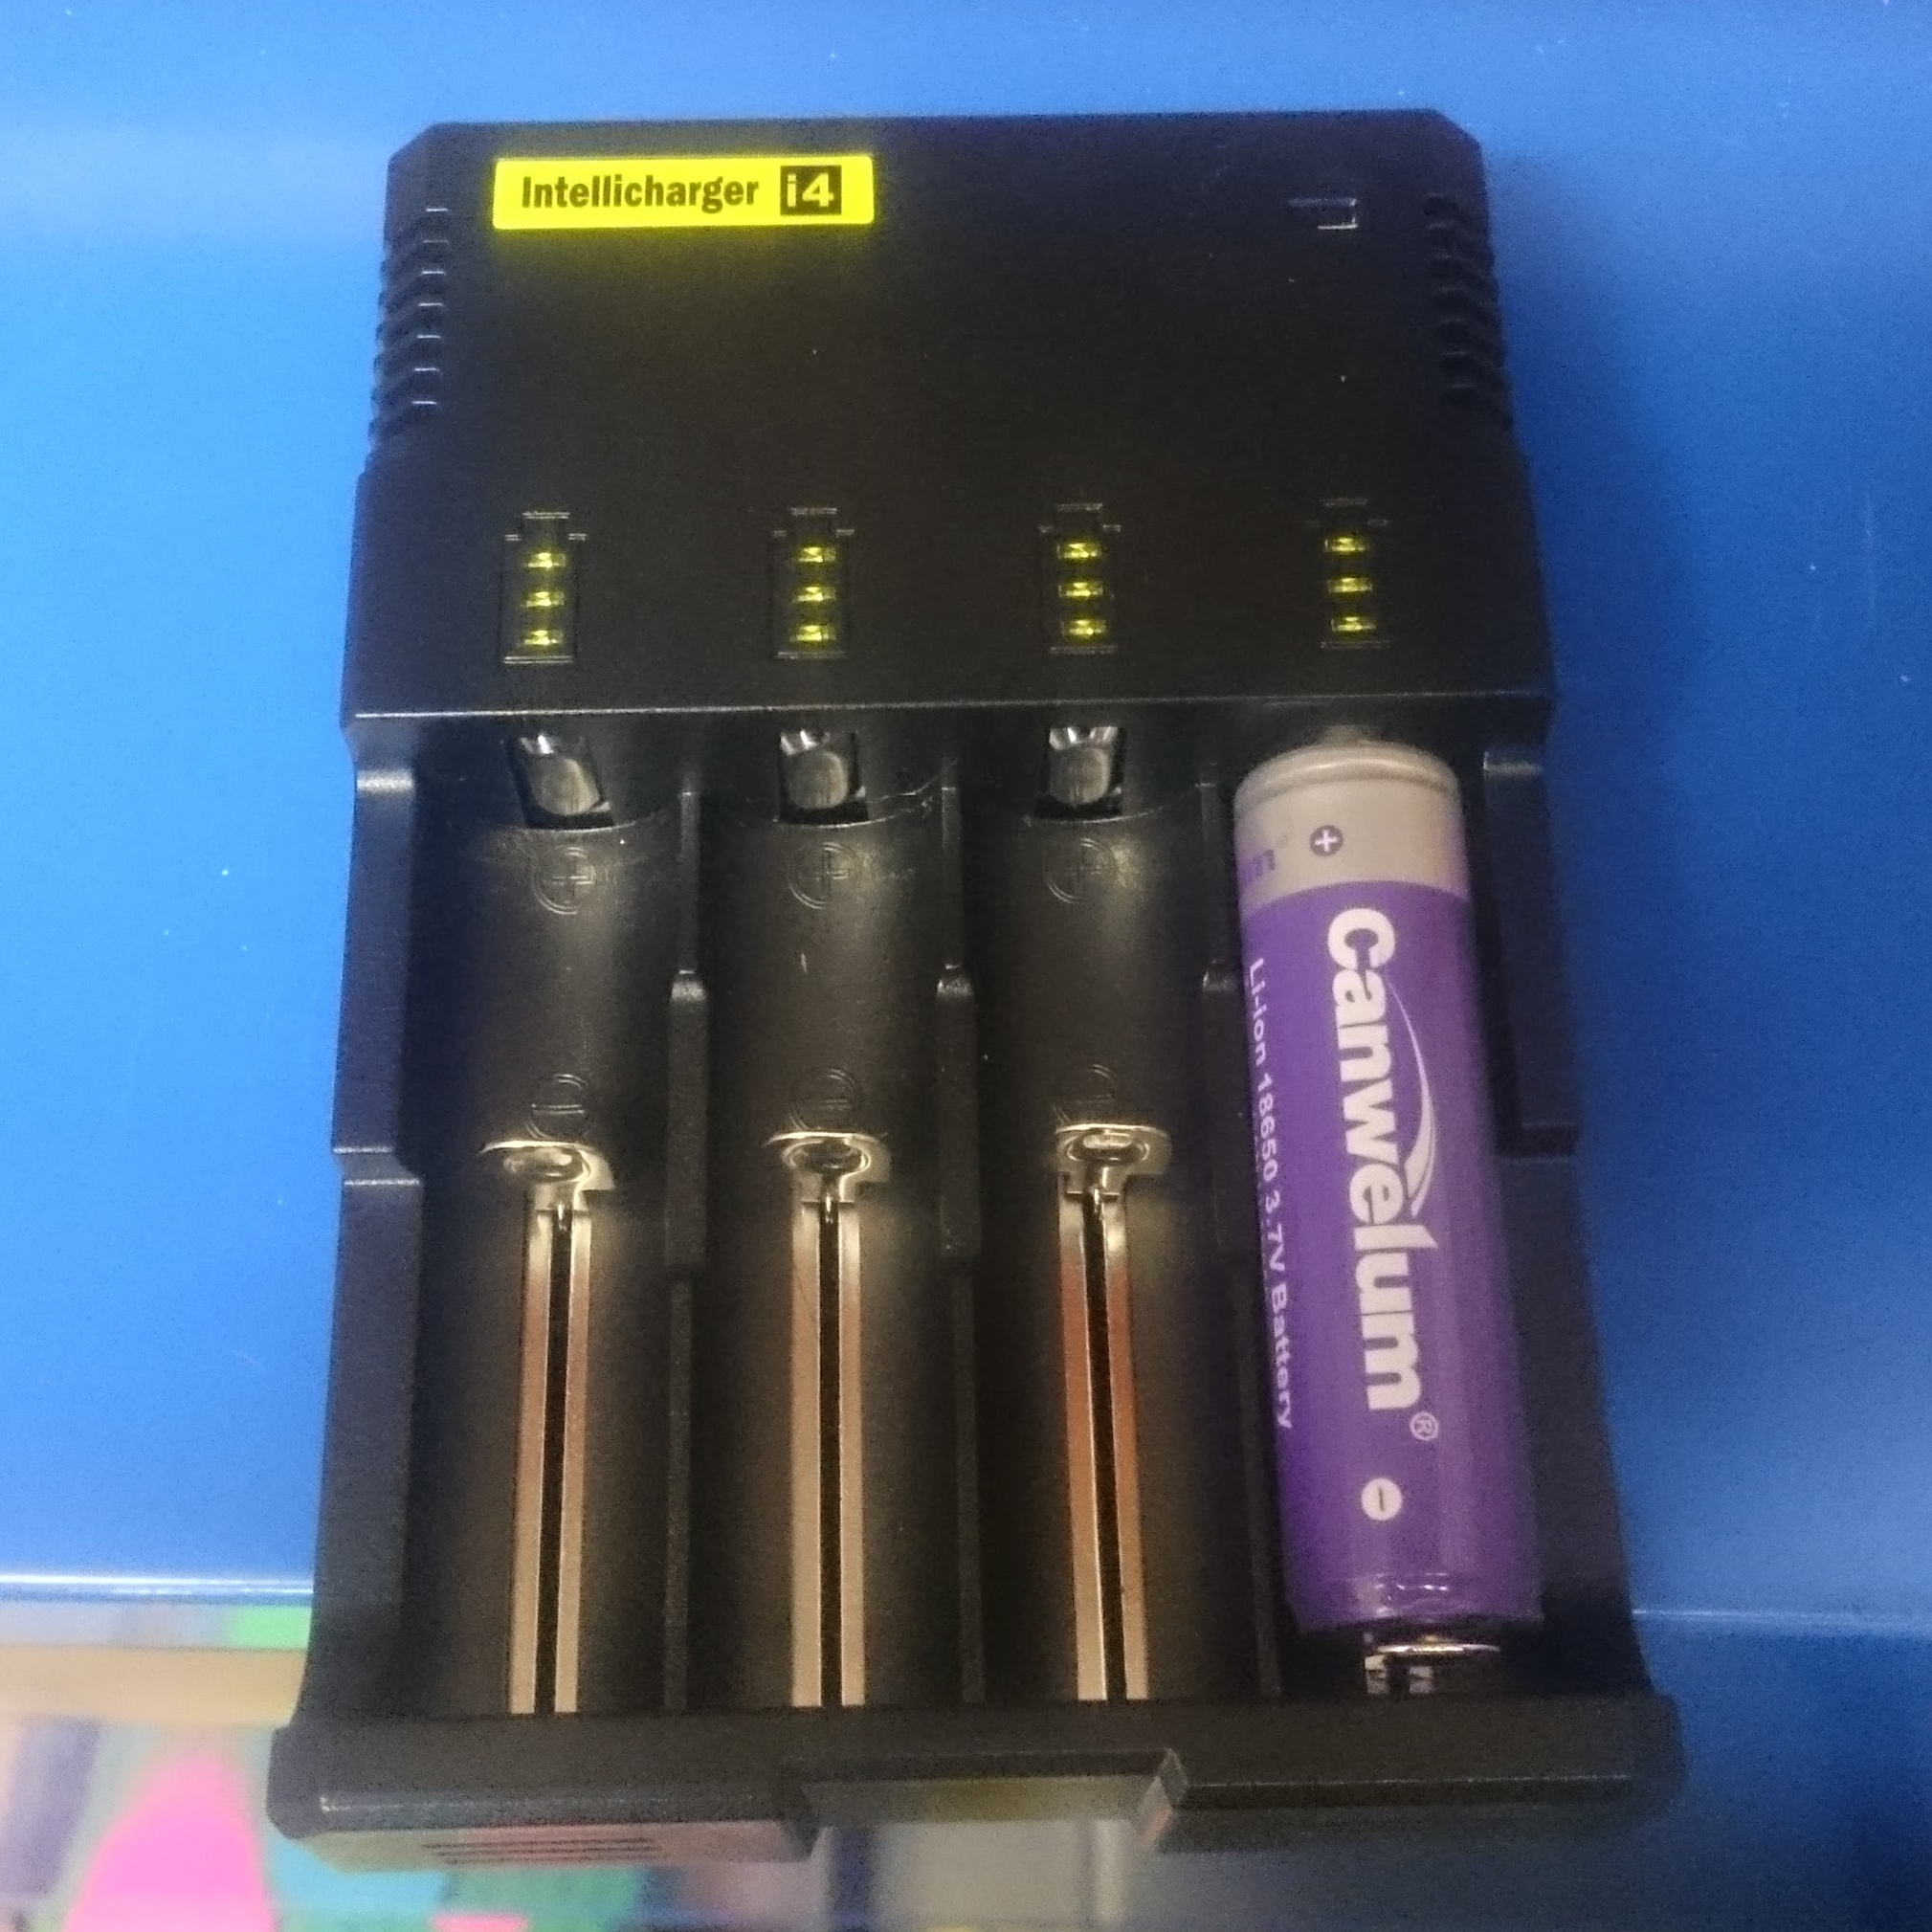
\includegraphics[width=.95\textwidth]{DSC_0147.jpg}
\caption{Charger With Correctly Oriented Cell}
\label{fig:charger}
\end{subfigure}
\caption{Hardware Pictures}
\label{fig:pics}
\end{figure}


\subsection{Turning the robot on}
Flip the switch towards the front of the robot, the robot will calibrate the grabbers by opening and closing them, and will then begin listening for commands.


\subsection{Changing the Power Cells}
\subsubsection{How to Change}
Start by switching off the robot by flicking the yellow switch away from the robot (as in \autoref{fig:robot_side}). The cells are held on by the externally accessible battery packs and can removed by gently pulling the batteries out of the packs (exactly as an AA cell is removed). New batteries should be inserted into the robot with the flat side against the springs. 2 sets of cells are provided so that one set can be charged while the robot is in use. The correctly inserted cells are visible in purple and silver in \autoref{fig:robot_side}.

\subsubsection{When to Change}
The voltage from the battery packs is regulated and should give the robot consistent performance. The cells include a built in low voltage cut off, to avoid issues from varying battery output. When any cell reaches the cut off, the robot will stop completely. At this point all the cells should be changed. 


\subsection{Charging}
The specialised charger (see \autoref{fig:charger}) can be used to recharge the batteries. If using a different charger, for safety and performance use a charger made for charging 18650 cells and ensure correct polarity.

The batteries should be placed into the charger with the flat side against the spring arm of the charger, as shown.
The charger shows a progress bar next to each cell. 

\section{Arduino Software}
\subsection{Sending commands}
In normal operation the commands should be sent through the planner with the \texttt{RFComms.py} module. 

For testing there is a \texttt{main\_manual.py} file which can be used to send individual commands to the robot by following the 
prompts, first for which RF stick to use and then a choice of commands. To see the entire command set  with descriptions hit `h' then enter at the prompt. 


\subsection{Command Response}
In response to a command the robot will first send an acknowledgment packet. It will then complete grab, release or kick commands, in order to leave the robot in a predictable state for the planner, then complete the given command. Move and turn commands are immediately dropped in order to use the new command. 

\subsection{Command Set}
\begin{table}[H]
\begin{tabularx}{\textwidth}{ llX }
\toprule
\textbf{Command} & \textbf{Arguments} & \textbf{Effect} \\
\midrule
kick & distance in cm & kick the ball to the specified distance\\
grab & N/A & this will respond with ``BC" for ball caught or ``NC" for not caught. \\
release & N/A & this will respond with ``grabbersOpen" to update the planner that it does not currently have the ball. \\
turn & angle in deg & turn counter clockwise if angle positive, clockwise if negative\\
move & distance in mm & move forward if distance is positive or backward if negative \\
ping & N/A &  will respond with positions of motors according to rotary encoders, for debugging purposes \\
\bottomrule
\end{tabularx}
\caption{Available Commands}
\end{table}

\subsubsection{Kick}
The robot grabs the grabbers in hard in order to place the ball and push the piston back. It then releases the grabbers until they are open as far as possible without obstructing the wheels, it then kicks a time dependent on the distance required (ranging from 50-200ms in typical operation). Finally, it closes the grabbers fully for continued movement.

\subsubsection{Grab}
The robot closes the grabbers until they are fully closed or for 800ms whichever comes sooner. If the grabbers do not close fully it is determined there is a ball in the grabbers and ``BC" is sent to the planner, otherwise ``NC" is sent.  

\subsubsection{Release}
The grabbers are released until they are open as far as possible without touching the wheels. ``grabbers open" is then sent to the planner. 

\subsubsection{Turn}
The robot turns a distance specified in degrees, this is non-blocking. 

\subsubsection{Move}
The robot accelerates up to the calibrated speed and then maintains that speed until it has just enough time to decelerate to the desired distance. It will correct for drift in order to keep the robot moving in a straight line. If it finds something in its way with the ultrasound sensor while moving forward (positive distance) it will stop and respond ``something in the way"

\subsection{Troubleshooting}
\begin{table}[H]
\begin{tabularx}{\textwidth}{ >{\hsize=.5\hsize}X >{\hsize=.5\hsize}X X }
\toprule
\textbf{Symptom} &\textbf{Possible Cause} &\textbf{Possible Solution} \\
\midrule
Robot not moving, no acknowledgment & No power from battery packs & Ensure cells are:inserted correctly, charged, all present. Check wire from battery packs to power regulator board is connected. Check wire from power regulator board to motor board is connected.
\\
\midrule
Robot not moving-no acknowledgment     &Robot only listening over USB. & Turn robot off and on using switch 
\\
\midrule
Robot not moving-with acknowledgement  & No power to motor board  & Check connection from power regulator board in middle to motor board on left (black and red wire), check I2C cable from power regulator board to motor board (4 wire cable)
\\
\midrule
Robot moving but not kicking  & Kicker signal cable disconnected & Check white 2 wire cable is going into power regulator board into  Left side of furthest back slot on power regulator board. 
\\
\midrule
Robot moving, but not straight, or not stopping & Cannot communicate with rotary encoders& Check for message which says ``cannot communicate with encoder board". This implies the 4 wire I2C connection from power regulator board in middle to encoder board on right is disconnected, check that movement of each wheel and the grabbers can be detected by checking their position with the ping command, check that when commanded each motor is moving, if not the power cable to that motor is damaged.
\\
\midrule
Robot will not move forward & Something in the way of ultrasound sensor & Check for ``something in the way" message to confirm cause, to solve first check if ultrasound sensor has been displaced or if something has got in way, as a last resort the sensor can be disabled altogether by unplugging it.
\\ 
\bottomrule
\end{tabularx}
\caption{Possible Problems and Solutions}
\end{table}